\documentclass[12pt]{article}
\usepackage{amsmath, amssymb, amsthm}
\usepackage{mathtools}
\usepackage{graphicx}
\usepackage{float}
\usepackage{hyperref}
\usepackage{xcolor}
\usepackage{listings}
\usepackage{geometry}
\usepackage{algorithm}
\usepackage{algpseudocode}
\usepackage{tikz}
\usepackage{longtable}
\usepackage{tikz}
\usepackage{circuitikz}
\usepackage{comment}
\usepackage{MnSymbol}
\usepackage{physics}
\usepackage{minted}
\usepackage[section]{placeins}

\providecommand{\brak}[1]{\ensuremath{\left(#1\right)}}
\geometry{a4paper, margin=1in}

\title{Assignment 1\\Engineering Electromagnetics EE1204}
\author{Agamjot Singh \brak{\text{EE24BTECH11002}}\\IIT Hyderabad}
\date{\today}

\begin{document}
\maketitle

\subsection*{Q1}
    Two point charges of equal magnitude $q$ are positioned at $z = \pm d/2$. We aim to determine:
    \begin{enumerate}
        \item[(a)] The electric field everywhere on the $z$-axis.
        \item[(b)] The electric field everywhere on the $x$-axis.
        \item[(c)] The results of (a) and (b) if the charge at $z = -d/2$ is $-q$ instead of $+q$.
    \end{enumerate}

\subsection*{Solution 1}
(a) Given two charges $q_1$ and $q_2$ located at $(0,0,d/2)$ and $(0,0,-d/2)$ respectively, we calculate the electric field $\vec{E}$ at a point $(0,0,z)$.

\begin{figure}[!ht]
    \centering
    \resizebox{0.5\textwidth}{!}{%
        \begin{circuitikz}
            \tikzstyle{every node}=[font=\large]
            \draw [line width=0.2pt, ->, >=Stealth] (8,5.75) -- (8,12.75);
            \draw [line width=0.2pt, ->, >=Stealth] (5,9.25) -- (11.75,9.25);
            \draw [ line width=0.2pt ] (8,10.75) circle (0.25cm);
            \draw [ line width=0.2pt ] (8,8) circle (0.25cm);
            \draw [->, thick, >=Stealth] (8,9.25) -- (8,12);
            \node [font=\large] at (8.25,11.75) {$\vec{r}$};
            \node [font=\large] at (7.25,10.75) {$q$};
            \node [font=\large] at (7.25,8) {$q$};
            \node [font=\large] at (9.5,10.5) {$(0, 0, d/2)$};
            \node [font=\large] at (9.5,7.75) {$(0, 0, -d/2)$};
            \node [font=\large] at (7,12) {$(0, 0, z)$};
            \node at (8,12) [circ] {};
            \node [font=\large] at (11.75,9) {$x$};
            \node [font=\large] at (7.75,12.75) {$z$};
        \end{circuitikz}
        }%

        \label{fig:my_label}
        \caption{Charge distribution for part (a)}
\end{figure}
Let $\vec{r} = z \hat{k}$ and $k = \dfrac{1}{4 \pi \epsilon_0}$.

\textbf{Electric Field due to $q_1$}
\begin{align*}
\vec{E}_1 = k \frac{q_1}{\abs{\vec{r} - \vec{r}_1}^3} (\vec{r} - \vec{r}_1)
\end{align*}
Substituting $\vec{r}_1 = \frac{d}{2} \hat{k}$:
\begin{align*}
    \vec{E}_1 = k q_1 \frac{z - \frac{d}{2}}{\abs{z - \frac{d}{2}}^3} \hat{k}= k q_1 \frac{1}{\brak{z - \frac{d}{2}}^2} \frac{\brak{z - \frac{d}{2}}}{\abs{z - \frac{d}{2}}} \hat{k}
\end{align*}

\textbf{Electric Field due to $q_2$}
\begin{align*}
\vec{E}_2 = k \frac{q_2}{\abs{\vec{r} - \vec{r}_2}^3} (\vec{r} - \vec{r}_2)
\end{align*}
Substituting $\vec{r}_2 = -\frac{d}{2} \hat{k}$:
\begin{align*}
    \vec{E}_2 = k q_2 \frac{z + \frac{d}{2}}{\abs{z + \frac{d}{2}}^3} \hat{k} = k q_2 \frac{1}{\brak{z + \frac{d}{2}}^2} \frac{\brak{z + \frac{d}{2}}}{\abs{z + \frac{d}{2}}} \hat{k}
\end{align*}

By superposition principle:
\begin{align*}
    \vec{E} = \vec{E}_1 + \vec{E}_2
\end{align*}

\textbf{Case 1:} $z > d/2$
\begin{align*}
\vec{E} = k q_1 \frac{\hat{k}}{\brak{z - \frac{d}{2}}^2} + k q_2 \frac{\hat{k}}{\brak{z + \frac{d}{2}}^2}
\end{align*}
If $q_1 = q_2 = q$, then:
\begin{align*}
\vec{E} = k q \brak{\frac{1}{\brak{z - \frac{d}{2}}^2} + \frac{1}{\brak{z + \frac{d}{2}}^2}} \hat{k}
\end{align*}


\textbf{Case 2:} $-\frac{d}{2} < z < \frac{d}{2}$
\begin{align*}
\vec{E} = k q_1 \frac{-\hat{k}}{\brak{z - \frac{d}{2}}^2} + k q_2 \frac{\hat{k}}{\brak{z + \frac{d}{2}}^2}
\end{align*}
If $q_1 = q_2 = q$, then:
\begin{align*}
\vec{E} = k q \brak{\frac{1}{\brak{z + \frac{d}{2}}^2} - \frac{1}{\brak{z - \frac{d}{2}}^2}} \hat{k}
\end{align*}

\textbf{Case 3:} $z < -d/2$
\begin{align*}
\vec{E} = k q_1 \frac{-\hat{k}}{\brak{z - \frac{d}{2}}^2} + k q_2 \frac{-\hat{k}}{\brak{z + \frac{d}{2}}^2}
\end{align*}
If $q_1 = q_2 = q$, then:
\begin{align*}
\vec{E} = -k q \brak{\frac{1}{\brak{z - \frac{d}{2}}^2} + \frac{1}{\brak{z + \frac{d}{2}}^2}} \hat{k}
\end{align*}

(b) Let $\vec{r} = x \hat{i}$ and $k = \dfrac{1}{4 \pi \epsilon_0}$.
\begin{align*}
    \vec{E}_1 = k \frac{q_1}{\abs{\vec{r} - \vec{r}_1}^3} (\vec{r} - \vec{r}_1) = k q_1\frac{\brak{x\hat{i} - \frac{d}{2}\hat{k}}}{\brak{x^2 + \brak{\frac{d}{2}}^2}^\frac{3}{2}}\\
    \vec{E}_2 = k \frac{q_2}{\abs{\vec{r} - \vec{r}_2}^3} (\vec{r} - \vec{r}_2) = k q_2\frac{\brak{x\hat{i} + \frac{d}{2}\hat{k}}}{\brak{x^2 + \brak{\frac{d}{2}}^2}^\frac{3}{2}}
\end{align*}

\begin{figure}[!ht]
    \centering
    \resizebox{0.5\textwidth}{!}{%
        \begin{circuitikz}
            \tikzstyle{every node}=[font=\large]
            \draw [line width=0.2pt, ->, >=Stealth] (8,5.75) -- (8,12.75);
            \draw [line width=0.2pt, ->, >=Stealth] (5,9.25) -- (11.75,9.25);
            \draw [ line width=0.2pt ] (8,10.75) circle (0.25cm);
            \draw [ line width=0.2pt ] (8,8) circle (0.25cm);
            \draw [->, thick, >=Stealth] (8,9.25) -- (10.75,9.25);
            \node [font=\large] at (10.75, 9) {$\vec{r}$};
            \node [font=\large] at (7.25,10.75) {$q$};
            \node [font=\large] at (7.25,8) {$q$};
            \node [font=\large] at (9.5,10.5) {$(0, 0, d/2)$};
            \node [font=\large] at (9.5,7.75) {$(0, 0, -d/2)$};
            \node [font=\large] at (11,9.55) {$(0, 0, x)$};
            \node at (10.75,9.25) [circ] {};
            \node [font=\large] at (11.75,8.75) {$x$};
            \node [font=\large] at (7.75,12.75) {$z$};
        \end{circuitikz}
        }%

        \label{fig:my_label}
        \caption{Charge distribution for part (a)}
\end{figure}

By superposition principle:
\begin{align*}
    \vec{E} &= \vec{E}_1 + \vec{E}_2
\end{align*}
Taking $q_1 = q_2 = q$,
\begin{align*}
    \vec{E} &= kq\frac{\brak{x\hat{i} - \frac{d}{2}\hat{k}}}{\brak{x^2 + \brak{\frac{d}{2}}^2}^\frac{3}{2}} + kq\frac{\brak{x\hat{i} + \frac{d}{2}\hat{k}}}{\brak{x^2 + \brak{\frac{d}{2}}^2}^\frac{3}{2}}\\
    \vec{E} &= 2kq \frac{x\hat{i}}{\brak{x^2 + \brak{\frac{d}{2}}^2}^\frac{3}{2}}
\end{align*}

(c) \textbf{Field on} $z$\textbf{-axis}
\newline
Charge distribution is same as that in part (a) and (b), except charge $q_2 = -q$.
From part (a):
\newline
\textbf{Case 1:} $z > d/2$
\begin{align*}
\vec{E} = k q_1 \frac{\hat{k}}{\brak{z - \frac{d}{2}}^2} + k q_2 \frac{\hat{k}}{\brak{z + \frac{d}{2}}^2}
\end{align*}
If $q_1 = q, q_2 = -q$, then:
\begin{align*}
\vec{E} = k q \brak{\frac{1}{\brak{z - \frac{d}{2}}^2} - \frac{1}{\brak{z + \frac{d}{2}}^2}} \hat{k}
\end{align*}

\textbf{Case 2:} $-\frac{d}{2} < z < \frac{d}{2}$
\begin{align*}
\vec{E} = k q_1 \frac{-\hat{k}}{\brak{z - \frac{d}{2}}^2} + k q_2 \frac{\hat{k}}{\brak{z + \frac{d}{2}}^2}
\end{align*}
If $q_1 = q, q_2 = -q$, then:
\begin{align*}
\vec{E} = -kq \brak{\frac{1}{\brak{z - \frac{d}{2}}^2} + \frac{1}{\brak{z + \frac{d}{2}}^2}} \hat{k}
\end{align*}

\textbf{Case 3:} $z < -d/2$
\begin{align*}
\vec{E} = k q_1 \frac{-\hat{k}}{\brak{z - \frac{d}{2}}^2} + k q_2 \frac{-\hat{k}}{\brak{z + \frac{d}{2}}^2}
\end{align*}
If $q_1 = q, q_2 = -q$, then:
\begin{align*}
\vec{E} = -k q \brak{\frac{1}{\brak{z - \frac{d}{2}}^2} - \frac{1}{\brak{z + \frac{d}{2}}^2}} \hat{k}
\end{align*}

\textbf{Field on} $x$\textbf{-axis}
\newline
Let $\vec{r} = x \hat{i}$ and $k = \dfrac{1}{4 \pi \epsilon_0}$.
\begin{align*}
    \vec{E}_1 = k \frac{q_1}{\abs{\vec{r} - \vec{r}_1}^3} (\vec{r} - \vec{r}_1) = k q_1\frac{\brak{x\hat{i} - \frac{d}{2}\hat{k}}}{\brak{x^2 + \brak{\frac{d}{2}}^2}^\frac{3}{2}}\\
    \vec{E}_2 = k \frac{q_2}{\abs{\vec{r} - \vec{r}_2}^3} (\vec{r} - \vec{r}_2) = k q_2\frac{\brak{x\hat{i} + \frac{d}{2}\hat{k}}}{\brak{x^2 + \brak{\frac{d}{2}}^2}^\frac{3}{2}}
\end{align*}

By superposition principle:
\begin{align*}
    \vec{E} &= \vec{E}_1 + \vec{E}_2
\end{align*}
Taking $q_1 = q, q_2 = -q$,
\begin{align*}
    \vec{E} &= kq\frac{\brak{x\hat{i} - \frac{d}{2}\hat{k}}}{\brak{x^2 + \brak{\frac{d}{2}}^2}^\frac{3}{2}} - kq\frac{\brak{x\hat{i} + \frac{d}{2}\hat{k}}}{\brak{x^2 + \brak{\frac{d}{2}}^2}^\frac{3}{2}}\\
    \vec{E} &= -kq \frac{d\hat{k}}{\brak{x^2 + \brak{\frac{d}{2}}^2}^\frac{3}{2}}
\end{align*}

\subsection*{Q2}
A crude device for measuring charge consists of two small insulating spheres of radius $a$, one of which is fixed in position. The other is movable along the x-axis and is subject to a restraining force $kx$, where $k$ is a spring constant. The uncharged spheres are centered at $x = 0$ and $x = d$, the latter fixed. If the spheres are given equal and opposite charges of $Q$ C, obtain the expression by which $Q$ may be found as a function of $x$. Determine the maximum charge that can be measured in terms of $\epsilon_0$, $k$, and $d$, and then state the separation of the spheres. What happens if a larger charge is applied?
\subsection*{Solution 2}
\begin{figure}[!ht]
\centering
\resizebox{0.6\textwidth}{!}{%
\begin{circuitikz}
\tikzstyle{every node}=[font=\large]
\draw (4.5,8.75) to[L ] (8.25,8.75);
\node at (4.5,8.75) [circ] {};
\draw  (8.25,8.75) circle (0.75cm);
\node at (8.25,8.75) [circ] {};
\draw  (11.5,8.75) circle (0.75cm);
\node at (11.5,8.75) [circ] {};
\draw [<->, >=Stealth] (4.5,7.25) -- (8.25,7.25);
\draw [<->, >=Stealth] (4.5,10.25) -- (11.5,10.25);
\node [font=\large] at (12.5,9.5) {$Q$};
\node [font=\large] at (9.25,9.5) {$-Q$};
\node [font=\normalsize] at (8.25,9.25) {$a$};
\node [font=\normalsize] at (11.5,9.25) {$a$};
\draw [->, >=Stealth] (8.25,8.75) -- (8.75,9.25);
\draw [->, >=Stealth] (11.5,8.75) -- (12,9.25);
\node [font=\large] at (6.32,9.5) {$k$};
\node [font=\large] at (6.25,6.9) {$x$};
\node [font=\large] at (7.5,10.75) {$d$};
\end{circuitikz}
}%

\label{fig:my_label}
\end{figure}

The forces acting on the movable sphere include the electrostatic force due to Coulomb's law and the restoring force due to the spring. At equilibrium, the net force on the left sphere $= 0$.

The electrostatic force on $-Q$ sphere due to $Q$ sphere with position vectors $\vec{r}_1$ and $\vec{r}_2$ respectively is given by,

\begin{align*}
F_e &= \frac{1}{4\pi \varepsilon_0} \frac{Q_1 Q_2}{\abs{\vec{r}_1 - \vec{r}_2}^3} \brak{\vec{r}_1 - \vec{r}_2}\\
\implies F_e &= -\frac{1}{4\pi \varepsilon_0} \frac{Q^2}{\abs{\vec{r}_1 - \vec{r}_2}^3} \brak{\vec{r}_1 - \vec{r}_2}
\end{align*}
In this case, $\vec{r}_1 = x \hat{i}$, $\vec{r}_2 = d \hat{i}$,
\begin{align*}
    F_e &= -\frac{1}{4\pi \varepsilon_0} \frac{Q^2}{\abs{d - x}^3} \brak{x\hat{i} - d\hat{i}}\\
    F_e &= \frac{1}{4\pi \varepsilon_0} \frac{Q^2}{\brak{d - x}^2} \hat{i} \text{ , } x < d
\end{align*}

The restoring force due to the spring on the $-Q$ charge is given by,
\begin{align}
F_s &= -k\vec{r}_1 = -kx \hat{i}
\end{align}
At equilibrium, net force on the $-Q$ charge $= 0$.

\begin{align*}
    -kx\hat{i} + \frac{Q^2}{4\pi\epsilon_0 (d-x)^2} \hat{i} &= 0 \\
    \frac{Q^2}{4\pi\epsilon_0 (d-x)^2} &= kx \\
    \implies Q = \sqrt{k(4\pi\epsilon_0)x(d-x)^2}
\end{align*}

To determine the maximum charge measurable, we differentiate $Q$ with respect to $x$ and find the maxima $\brak{0 < x < \frac{d}{2}}$.

\begin{align*}
    \frac{dQ}{dx} = \sqrt{4k\pi\epsilon_0} \left( \frac{1}{2 \sqrt{x(d-x)^2}} \right) \left( -2x(d-x) + (d-x)^2 \right) = 0 \\
\end{align*}
\begin{align*}
\Rightarrow -2x(d-x) + (d-x)^2 &= 0 \\
\Rightarrow (d-x)(-2x + d - x) &= 0 \\
\Rightarrow (d-x)(d-3x) &= 0 \\
\Rightarrow x = d &\text{ or } x = \frac{d}{3}
\end{align*}

So, $x = \frac{d}{3}$ is the maxima. 
\begin{align*}
    Q &= \sqrt{k(4\pi\epsilon_0)x\brak{d-x}^2}\\
    Q_{max} &= \sqrt{k(4\pi\epsilon_0)\frac{d}{3}\brak{\frac{2d}{3}}^2}\\
    \implies Q_{max} &= \frac{4d}{3}\sqrt{k\pi\epsilon_0 \frac{d}{3}}\\
\end{align*}
The separation between the spheres when $Q = Q_{max}$ is equal to $d - x = \frac{2d}{3}$

\textbf{Behavior for Larger Charges}
\newline
As the charge $Q$ increases and goes beyond $Q_{max}$, the equilibrium point $x > d$, which implies that the spheres will come in contact and collide before the $-Q$ sphere can even reach equilibrium.
\newline
Due to this limitation, this measuring device is not that effective in practical scenarios.

\subsection*{Q3}
A flux density field is given as
\begin{align*}
\mathbf{F_1} = 5\mathbf{a_z}.
\end{align*}
The task is to evaluate the outward flux of $\mathbf{F_1}$ through the hemispherical surface defined by $r = a$, $0 < \theta < \pi/2$, and $0 < \phi < 2\pi$. Next, consider what simple observation would have saved a lot of work in the previous part. Identifying symmetries or using alternative methods can simplify the calculations significantly. Now suppose the field is given by

\begin{align*}
\mathbf{F_2} = 5z\mathbf{a_z}.
\end{align*}

Using the appropriate surface integrals, determine the net outward flux of $\mathbf{F_2}$ through the closed surface consisting of the hemisphere from the first part and its circular base in the $xy$ plane. Finally, repeat the previous calculation by applying the divergence theorem and evaluating an appropriate volume integral. This approach should confirm the result obtained through direct surface integration.

\subsection*{Solution 3}
\begin{figure}[!ht]
    \begin{center}
        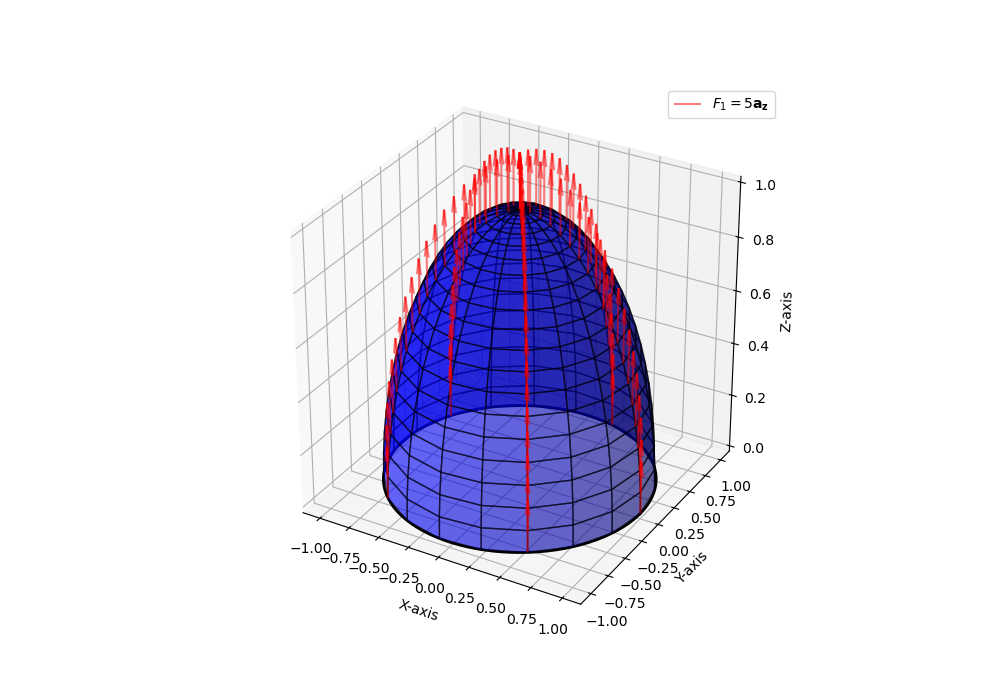
\includegraphics[width=0.95\textwidth]{./q3/fig.png}
    \end{center}
    \caption{""}
\end{figure}

We solve this question in spherical coordinate system. 
Converting $\mathbf{a_z}$ to spherical system,
\begin{align*}
    \mathbf{a_z} &= \brak{\cos{\theta}} \vec{r} - \brak{\sin{\theta}} \vec{\theta}\\
    \implies \mathbf{F_1} &= 5 \mathbf{a_z} = 5 \brak{\brak{\cos{\theta}} \vec{r} - \brak{\sin{\theta}} \vec{\theta}}
\end{align*}
Also,
\begin{align*}
    \hat{n}\; dS &= \brak{r^2\sin{\theta}\; d\phi \; d\theta} \hat{r}\\
    \implies \text{Flux} &= \iint \mathbf{F_1}\cdot\brak{\hat{n} \; dS}\\
    &= \iint 5 \brak{\brak{\cos{\theta}} \vec{r} - \brak{\sin{\theta}} \vec{\theta}} \cdot \brak{r^2\sin{\theta}\; d\phi \; d\theta} \hat{r}\\
    &= 5\int\limits_{\phi \;=\; 0}^{2\pi}\int\limits_{\theta \;=\; 0}^{\frac{\pi}{2}} r^2 \sin{\theta} \cos{\theta} \; d\phi \; d\theta\\
    &= 5a^2 \int\limits_{\phi \;=\; 0}^{2\pi}\int\limits_{\theta \;=\; 0}^{\frac{\pi}{2}} \sin{\theta} \cos{\theta} \; d\phi \; d\theta \text{ , } \brak{\text{as } r = a}\\
    &= 5a^2 \int\limits_{0}^{2\pi} \frac{1}{2} \; d\phi\\
    &= 5\pi a^2
\end{align*}

\textbf{An alternative easier method to solve:} \newline
Stoke's theorem implies that the flux of a field through a surface only depends on the closed boundary of the surface.
\begin{align*}
\oint_C \mathbf{F} \cdot d\mathbf{r} = \iint_S (\nabla \times \mathbf{F}) \cdot d\mathbf{S}
\end{align*}
The boundary of the hemispherical region is given by,
\begin{align*}
    C: x^2 + y^2 = a^2
\end{align*}
We are now going to take the circular surface bounded by this boundary as the new surface $S^\prime$. By Stoke's Theorem,
\begin{align*}
    \oint_C \mathbf{F} \cdot d\mathbf{r} = \iint_S (\nabla \times \mathbf{F}) \cdot d\mathbf{S} = \iint_{S^\prime} (\nabla \times \mathbf{F}) \cdot d\mathbf{S}
\end{align*}
Take $\brak{\nabla \times \mathbf{F}} = \mathbf{F_1}$, we get,
\begin{align*}
     \iint_S \mathbf{F_1} \cdot d\mathbf{S} = \iint_{S^\prime} \mathbf{F_1} \cdot d\mathbf{S}
\end{align*}

For $S^\prime$,
\begin{align*}
    \hat{n} &= \mathbf{a_z} \text{ } \brak{\text{in anticlockwise sense}}\\
    \iint_S \mathbf{F_1} \cdot d\mathbf{S} &= \iint \brak{5\mathbf{a_z}}\cdot\brak{\mathbf{a_z}} \; dS\\
    &= 5\iint dS\\
    &= 5\pi a^2
\end{align*}

\textbf{Net outward flux of} $\mathbf{F_2}$ \textbf{:}

Converting $\mathbf{a_z}$ and $\mathbf{F_2}$ to spherical system,
\begin{align*}
    \mathbf{a_z} &= \brak{\cos{\theta}} \vec{r} - \brak{\sin{\theta}} \vec{\theta}\\
    z &= r\cos{\theta}\\
    \implies \mathbf{F_2} &= 5 z\mathbf{a_z} = 5r\cos{\theta} \brak{\brak{\cos{\theta}} \vec{r} - \brak{\sin{\theta}} \vec{\theta}}
\end{align*}
Also, for outward flux through hemispherical region,
\begin{align*}
    \hat{n}\; dS &= \brak{r^2\sin{\theta}\; d\phi \; d\theta} \hat{r}\\
    \text{Flux through hemisphere} &= \iint \mathbf{F_2}\cdot\brak{\hat{n} \; dS}\\
    &= \iint 5r\cos{\theta} \brak{\brak{\cos{\theta}} \vec{r} - \brak{\sin{\theta}} \vec{\theta}} \cdot \brak{r^2\sin{\theta}\; d\phi \; d\theta} \hat{r}\\
    &= 5\int\limits_{\phi \;=\; 0}^{2\pi}\int\limits_{\theta \;=\; 0}^{\frac{\pi}{2}} r^3 \sin{\theta} \cos^2{\theta} \; d\phi \; d\theta\\
    &= 5a^3 \int\limits_{\phi \;=\; 0}^{2\pi}\int\limits_{\theta \;=\; 0}^{\frac{\pi}{2}} \sin{\theta} \cos^2{\theta} \; d\phi \; d\theta \text{ , } \brak{\text{as } r = a}\\
    &= 5a^3 \int\limits_{\phi \;=\; 0}^{2\pi}\int\limits_{\theta \;=\; 0}^{\frac{\pi}{2}} \brak{\sin{\theta} - \sin^3{\theta}} \; d\phi \; d\theta \text{ , } \brak{\text{as } r = a}\\
    &= 5a^3 \int\limits_{\phi \;=\; 0}^{2\pi}\int\limits_{\theta \;=\; 0}^{\frac{\pi}{2}} \frac{1}{4}\brak{\sin{3\theta} + \sin{\theta}} \; d\phi \; d\theta \text{ , } \brak{\text{as } r = a}\\
    &= 5a^3 \int\limits_{0}^{2\pi} \frac{1}{3} \; d\phi\\
    &= \frac{10}{3}\pi a^3
\end{align*}

Now we calculate the outward flux through the circular base in the $xy$ plane.
\begin{align*}
    \hat{n} &= -\mathbf{a_z} \text{ } \brak{\text{in clockwise sense for outward flux}}\\
    \iint \mathbf{F_2} \cdot \brak{\hat{n}\;dS} &= \iint \brak{5z\mathbf{a_z}}\cdot\brak{-\mathbf{a_z}} \; dS\\
    &= \iint 5z \; dS \\
    &= 0
\end{align*}
But the region lies on the $xy$ plane, so $z = 0$. So the outward flux through the circular base $= 0$.
\newline
Thus, the total outward flux through the closed volume $= \frac{10}{3}\pi a^3$.

\textbf{Using divergence theorem to calculate outward flux:}
Divergence theorem states that,
\begin{align*}
    \iiint_{D} (\nabla \cdot \mathbf{F}) \, dV = \oiint_{S} \mathbf{F} \cdot d\mathbf{S} 
\end{align*}
where $D$ is the volume enclosed by the surface $S$.
\newline
Let $\mathbf{F_2} = F_x \mathbf{a_x} + F_y \mathbf{a_y} + F_z \mathbf{a_z} \implies F_x = F_y = 0$, $F_z = 5z$.
\begin{align*}
    \nabla \cdot \mathbf{F_2} &= \frac{\partial F_x}{\partial x} + \frac{\partial F_y}{\partial y} + \frac{\partial F_z}{\partial z}\\
    \implies \nabla \cdot \mathbf{F_2} &= 5
\end{align*}

Substituting in divergence theorem,
\begin{align*}
    \text{Outward Flux through } S &= \oiint_{S} \mathbf{F} \cdot d\mathbf{S}\\
    &= \iiint_{D} (\nabla \cdot \mathbf{F}) \, dV\\
    &= 5 \iiint_{D} dV\\
    &= 5 \text{ (Volume enclosed by hemisphere)}\\
    &= 5 \brak{\frac{4}{3} \pi a^3 \times \frac{1}{2}}\\
    &= \frac{10}{3} \pi a^3
\end{align*}
The outward flux is same as that of previous calculations, without using divergence theorem. But it is clearly seen divergence theorem eases out the calculations by a lot.

\subsection*{Q4}
An infinitely long cylindrical dielectric of radius $b$ contains charge within its volume with a charge density given by
\begin{align*}
\rho_v = a\rho^2
\end{align*}
where $a$ is a constant. The goal is to determine the electric field strength $\mathbf{E}$ both inside and outside the cylinder.

\subsection*{Solution 4}
As the cylinder is infinitely long, and cylindrically symmetric charge distribution, electric field is always radially outwards. 

(a) Inside the cylinder $\brak{0 < \rho < b}$, we take a cylindrical gaussian surface with radius $\rho = r$ and length $l$.
\begin{figure}[!ht]
\centering
\resizebox{0.5\textwidth}{!}{%
\begin{circuitikz}
\tikzstyle{every node}=[font=\large]

\draw  (6.25,10.25) circle (2.5cm);
\draw [ dashed] (6.25,10.25) circle (1.5cm);
\node at (6.25,10.25) [circ] {};
\draw [->, >=Stealth] (6.25,10.25) -- (7,11.5);
\draw [->, >=Stealth] (6.25,10.25) -- (4.5,12);
\node [font=\large] at (5.25,10.75) {$b$};
\node [font=\large] at (7,10.75) {$r$};
\end{circuitikz}
}%

\label{fig:my_label}
\caption{Cross sectional view of the cylindrical dielectric, when $0 < r < b$}
\end{figure}
Charge enclosed is given by,
\begin{align*}
    Q_{enc} &= \iiint \rho_v \;dV\\
    &= \int\limits_{\theta \;=\; 0}^{2\pi} \int\limits_{z \;=\; 0}^{l} \int\limits_{\rho \;=\; 0}^{r} \brak{a\rho^2} \rho \;d\rho \;dz \;d\theta\\
    &= \int\limits_{\theta \;=\; 0}^{2\pi} \int\limits_{z \;=\; 0}^{l} \brak{\frac{a}{4}r^4}\;dz \;d\theta\\
    &= \frac{\pi}{2} alr^4
\end{align*}
Let $\mathbf{E} = E\hat{\rho}$. By Gauss's law,
\begin{align*}
    \oiint_S \mathbf{E}\cdot\brak{\hat{n}\;dS} &= \frac{Q_{enc}}{\epsilon_0} = \frac{\pi}{2\epsilon_0} alr^4\\
    \oiint_S \brak{E \hat{\rho}}\cdot\hat{\rho}\;dS &= \frac{\pi}{2\epsilon_0} alr^4\\
    E \oiint_S \;dS &= \frac{\pi}{2\epsilon_0} alr^4\\
    \implies E \brak{2\pi rl} &= \frac{\pi}{2\epsilon_0} alr^4\\
    \implies E &= \frac{ar^3}{4\epsilon_0}\\
    \mathbf{E} &=  \frac{ar^3}{4\epsilon_0} \hat{\rho}
\end{align*}
Substituting $r = \rho$ for getting in terms of cylindrical coordinates,
\begin{align*}
    \mathbf{E} &= \frac{a{\rho}^3}{4\epsilon_0} \hat{\rho} \text{ , } 0 < \rho < b
\end{align*}

(b) Outside the cylinder \brak{\rho > b},
\begin{figure}[!ht]
\centering
\resizebox{0.5\textwidth}{!}{%
\begin{circuitikz}
\tikzstyle{every node}=[font=\large]

\draw  (6.25,10.25) circle (2.5cm);
\node at (6.25,10.25) [circ] {};
\draw [->, >=Stealth] (6.25,10.25) -- (4.5,12);
\node [font=\large] at (5.25,10.75) {b};
\draw [ dashed] (6.25,10.25) circle (4.25cm);
\draw [->, >=Stealth] (6.25,10.25) -- (9.25,13);
\node [font=\large] at (7.75,11.25) {$\rho$};
\end{circuitikz}
}%

\label{fig:my_label}
\caption{Cross sectional view of the cylindrical dielectric, when $\rho > b$}
\end{figure}
\begin{align*}
    Q_{enc} = \frac{\pi}{2} alb^4
\end{align*}
Let $\mathbf{E} = E\hat{\rho}$. By Gauss's law,
\begin{align*}
    \oiint_S \mathbf{E}\cdot\brak{\hat{n}\;dS} &= \frac{Q_{enc}}{\epsilon_0} = \frac{\pi}{2\epsilon_0} alb^4\\
    \oiint_S \brak{E \hat{\rho}}\cdot\hat{\rho}\;dS &= \frac{\pi}{2\epsilon_0} alb^4\\
    E \oiint_S \;dS &= \frac{\pi}{2\epsilon_0} alb^4\\
    \implies E \brak{2\pi \rho l} &= \frac{\pi}{2\epsilon_0} alb^4\\
    \mathbf{E} &=  \frac{ab^4}{4\rho\epsilon_0} \hat{\rho}
\end{align*}

\subsection*{Q5}
Given the vector field in cylindrical coordinates:
\begin{align}
\vec{F} = \left[ \frac{40}{s^2 + 1} + 3(\cos \phi + \sin \phi) \right] \hat{s} + 3(\cos \phi - \sin \phi) \hat{\phi} - 2\hat{z}
\end{align}

\begin{enumerate}
    \item[(a)] Compute and plot the magnitude $|\vec{F}|$ as a function of $\phi$ for $s = 3$.
    \item[(b)] Compute and plot the magnitude $|\vec{F}|$ as a function of $s$ for $\phi = 45^\circ$.
    \item[(c)] Calculate the divergence $\nabla \cdot \vec{F}$.
    \item[(d)] Calculate the curl $\nabla \times \vec{F}$ and verify whether the field is conservative.
\end{enumerate}

\subsection*{Solution 5}
(a) The magnitude of $\vec{F} = F_s \hat{s} + F_\phi \hat{\phi} + F_z \hat{z}$ is given by,
\begin{align*}
    \abs{\vec{F}} &= \sqrt{F_s^2 + F_\phi^2 + F_z^2}\\
    &= \sqrt{ \brak{\frac{40}{s^2 + 1} + 3(\cos \phi + \sin \phi)}^2 + \brak{3\brak{\cos \phi - \sin \phi}}^2 + 4}
\end{align*}
For $s = 3$,
\begin{align*}
    \abs{\vec{F}} &= \sqrt{\brak{8 + 3 \sin{\phi} + 3\cos{\phi}}^2 + \brak{3\cos{\phi} - 3\sin{\phi}}^2 + 4}\\
    &= \sqrt{38 + 24\brak{\cos{\phi} + \sin{\phi}}}
\end{align*}

\begin{figure}[!ht]
    \begin{center}
        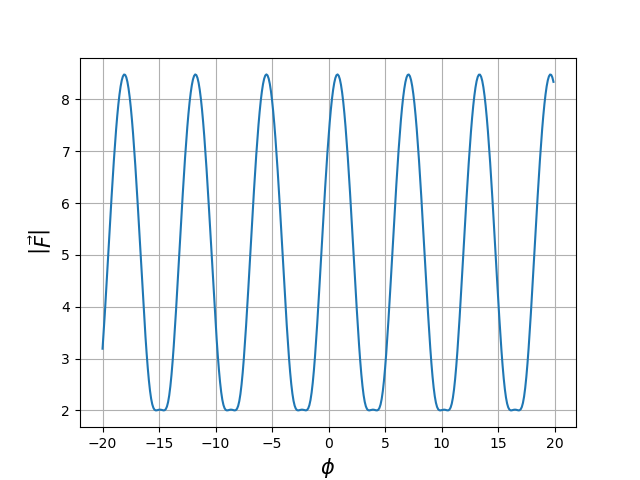
\includegraphics[width=0.5\textwidth]{./q5/a_fig.png}
    \end{center}
    \caption{Magnitude of $\vec{F}$ vs $\phi$, given s = 3}
\end{figure}

(b) For $\phi = 45\deg$,
\begin{align*}
    \abs{\vec{F}} &= \sqrt{\brak{\frac{40}{s^2 + 1} + 3\sqrt{2}}^2 + 4}
\end{align*}
\newpage

\begin{figure}[!ht]
    \begin{center}
        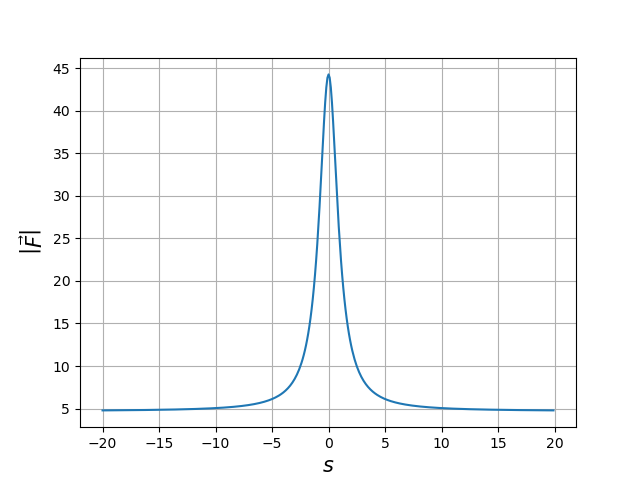
\includegraphics[width=0.6\textwidth]{./q5/b_fig.png}
    \end{center}
    \caption{Magnitude of $\vec{F}$ vs $s$, given $\phi = \pi/4$}
\end{figure}

(c) Divergence of $\vec{F}$ in cylindrical coordinates is given by,
\begin{align*}
    \nabla \cdot \vec{F} &= \frac{1}{s} \frac{\partial \brak{s F_s}}{\partial s} + \frac{1}{s} \frac{\partial \brak{F_{\phi}}}{\partial \phi} + \frac{\partial F_z}{\partial z}
\end{align*}

Note that,
\begin{align*}
    \vec{F} &= F_s \hat{s} + F_{\phi} \hat{\phi} + F_z \hat{z}\\
    \implies F_s &= \frac{40}{s^2 + 1} + 3\brak{\cos{\phi} + \sin{\phi}}\\
    F_{\phi} &= 3\brak{\cos{\phi} - \sin{\phi}}\\
    F_z &= -2
\end{align*}

Divergence of $\vec{F}$ is now given by,
\begin{align*}
    \nabla \cdot \vec{F} &= \frac{1}{s} \frac{\partial \brak{\brak{\frac{40s}{s^2 + 1}} + 3s\brak{\cos{\phi} + \sin{\phi}}}}{\partial s} + \frac{1}{s} \frac{\partial \brak{3\brak{\cos{\phi} - \sin{\phi}}}}{\partial \phi} + \frac{\partial \brak{-2}}{\partial z}\\
    &= \frac{1}{s} \brak{40\frac{1 - s^2}{\brak{1 + s^2}^2} + 3\brak{\cos{\phi} + \sin{\phi}}} - \frac{3}{s} \brak{\sin{\phi} + \cos{\phi}}\\
    &= 40\brak{\frac{1 - s^2}{s\brak{1 + s^2}^2}}
\end{align*}

(d) Curl of $\vec{F}$ in spherical coordinates is given by,
\begin{align*}
\nabla \times \vec{F} &= \left( \frac{1}{s} \frac{\partial F_z}{\partial \phi} - \frac{\partial F_\phi}{\partial z} \right) \hat{s}
+ \left( \frac{\partial F_s}{\partial z} - \frac{\partial F_z}{\partial s} \right) \hat{\phi}
+ \frac{1}{s} \left( \frac{\partial (s F_\phi)}{\partial s} - \frac{\partial F_s}{\partial \phi} \right) \hat{z}
\end{align*}

As $F_z = $ constant,
\begin{align*}
    \frac{\partial F_z}{\partial \phi} &= \frac{\partial F_z}{\partial s} = \frac{\partial F_z}{\partial z} = 0\\
\end{align*}

As $F_s$ and $F_{\phi}$ are independent of $z$,
\begin{align*}
    \frac{\partial F_s}{\partial z} &= \frac{\partial F_{\phi}}{\partial z} = 0
\end{align*}

Also,
\begin{align*}
    \frac{\partial \brak{s F_{\phi}}}{\partial z} &= \frac{\partial \brak{3s\brak{\cos{\phi} - \sin{\phi}}}}{\partial z} = 3\brak{\cos{\phi} - \sin{\phi}}\\
    \frac{\partial F_s}{\partial \phi} &= 3\brak{\cos{\phi} - \sin{\phi}}\\
    \implies \brak{ \frac{\partial (s F_\phi)}{\partial s} - \frac{\partial F_s}{\partial \phi} } &= 0
\end{align*}

Substituting in the curl expression,
\begin{align*}
    \nabla \times \vec{F} = 0
\end{align*}

By Stokes's theorem,
\begin{align*}
    \oint_C \vec{F} \cdot d\vec{r} = \iint_S (\nabla \times \vec{F}) \cdot d\vec{S} &= 0\\
    \implies \text{Line integral of } \vec{F} \text{ in a closed loop} &= 0
\end{align*}
That implies that $\vec{F}$ is a conservative field.

\subsection*{Q6}
Refer the charge distribution given in the assignment paper, solve the following:

\begin{enumerate}
    \item[(a)] Plot the Electric Field.
    \item[(b)] Plot the potential with magnitude represented along the Z-axis.
    \item[(c)] Compute the potential energy of the configuration.
    \item[(d)] Use Gauss's Law to verify the divergence of the electric field.
    \item[(e)] Verify whether the curl of the electric field is zero.
\end{enumerate}

\subsection*{Solution 6}
(a) Let $\vec{r} = x\hat{i} + y\hat{j}$,
\begin{align*}
    \vec{E}_1 &= \frac{1}{4\pi\epsilon_0} \frac{q}{\abs{\vec{r} - \vec{r_1}}^3} \brak{\vec{r} - \vec{r_1}} = \frac{1}{4\pi\epsilon_0} \frac{q}{\brak{x^2 + \brak{y - 1}^2}^{\frac{3}{2}}} \brak{x\hat{i} + \brak{y - 1} \hat{j}}\\
    \vec{E}_2 &= \frac{1}{4\pi\epsilon_0} \frac{q}{\abs{\vec{r} - \vec{r_2}}^3} \brak{\vec{r} - \vec{r_2}} = \frac{1}{4\pi\epsilon_0} \frac{q}{\brak{x^2 + \brak{y + 1}^2}^{\frac{3}{2}}} \brak{x\hat{i} + \brak{y + 1} \hat{j}}\\
    \vec{E}_3 &= \frac{1}{4\pi\epsilon_0} \frac{q}{\abs{\vec{r} - \vec{r_3}}^3} \brak{\vec{r} - \vec{r_3}} = -\frac{1}{4\pi\epsilon_0} \frac{1}{\brak{\brak{x - 1}^2 + y^2}^{\frac{3}{2}}} \brak{\brak{x - 1}\hat{i} + y\hat{j}}\\
    \vec{E}_4 &= \frac{1}{4\pi\epsilon_0} \frac{q}{\abs{\vec{r} - \vec{r_4}}^3} \brak{\vec{r} - \vec{r_4}} = -\frac{1}{4\pi\epsilon_0} \frac{1}{\brak{\brak{x + 1}^2 + y^2}^{\frac{3}{2}}} \brak{\brak{x + 1}\hat{i} + y\hat{j}}
\end{align*}
Note that,
\begin{align*}
    \vec{r_1} = \hat{j}\\
    \vec{r_2} = -\hat{j}\\
    \vec{r_3} = \hat{i}\\
    \vec{r_3} = -\hat{i}
\end{align*}
By superposition principle,
\begin{align*}
    \vec{E} = \vec{E_1} + \vec{E_2} + \vec{E_3} + \vec{E_4}
\end{align*}

\begin{figure}
    \begin{center}
        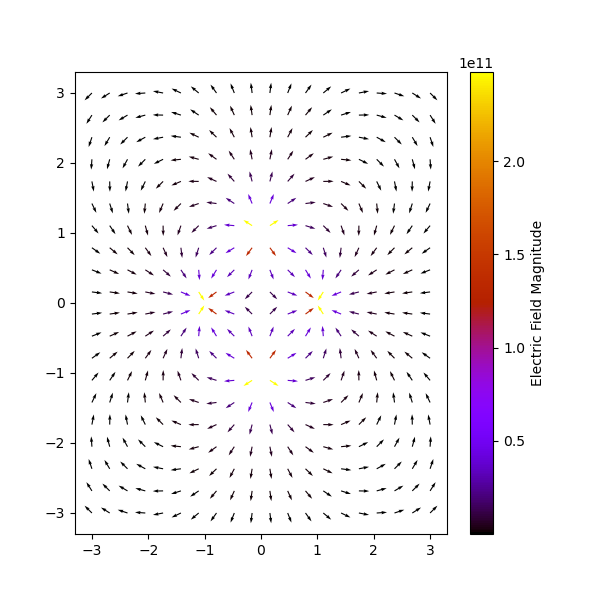
\includegraphics[width=0.5\textwidth]{./q6/a_fig.png}
    \end{center}
    \caption{Field plot of $\vec{E}$}
\end{figure}


(b) Let $\vec{r} = x\hat{i} + y\hat{j}$,
\begin{align*}
    V_1 &= \frac{1}{4\pi\epsilon_0} \frac{q}{\abs{\vec{r} - \vec{r_1}}}  = \frac{1}{4\pi\epsilon_0} \frac{1}{\brak{x^2 + \brak{y - 1}^2}^{\frac{1}{2}}}\\
    V_2 &= \frac{1}{4\pi\epsilon_0} \frac{q}{\abs{\vec{r} - \vec{r_2}}}  = \frac{1}{4\pi\epsilon_0} \frac{1}{\brak{x^2 + \brak{y + 1}^2}^{\frac{1}{2}}}\\
    V_3 &= \frac{1}{4\pi\epsilon_0} \frac{q}{\abs{\vec{r} - \vec{r_3}}}  = \frac{1}{4\pi\epsilon_0} \frac{1}{\brak{\brak{x - 1}^2 + y^2}^{\frac{1}{2}}}\\
    V_4 &= \frac{1}{4\pi\epsilon_0} \frac{q}{\abs{\vec{r} - \vec{r_4}}}  = \frac{1}{4\pi\epsilon_0} \frac{1}{\brak{\brak{x + 1}^2 + y^2}^{\frac{1}{2}}}
\end{align*} 
By superposition theorem,
\begin{align*}
    V = V_1 + V_2 + V_3 + V_4
\end{align*}
\newpage

\begin{figure}
    \begin{center}
        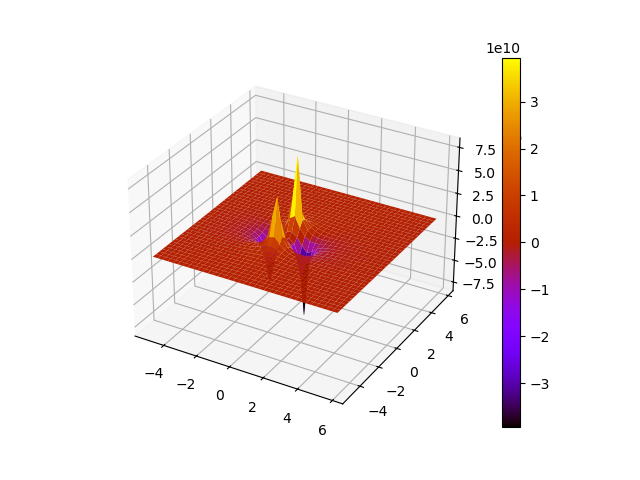
\includegraphics[width=0.5\textwidth]{./q6/b_fig.png}
    \end{center}
    \caption{Potential Field plot}
\end{figure}

(c) Potential energy of a discrete charge distribution is given by,
\begin{align*}
    U = \frac{1}{4\pi\epsilon_0} \sum\limits_{i < j} \frac{Q_i Q_j}{\abs{\vec{r_i} - \vec{r_j}}}
\end{align*}
For the given distribution,
\begin{align*}
    U &= \frac{1}{4\pi\epsilon_0} \brak{  \frac{\brak{1}\brak{-1}}{\sqrt{2}} + \frac{\brak{1}\brak{1}}{2} + \frac{\brak{1}\brak{-1}}{\sqrt{2}} + \frac{\brak{1}\brak{-1}}{\sqrt{2}} + \frac{\brak{-1}\brak{-1}}{2} +  \frac{\brak{-1}\brak{1}}{\sqrt{2}} }\\
    \implies U &= \frac{1}{4\pi\epsilon_0} \brak{1 - 2\sqrt{2}} 
\end{align*}

(d) Say a charge of magnitude $Q$ is placed in the $xy$ plane at origin.
\begin{align*}
    \nabla \cdot \mathbf{E} &= \nabla \cdot \brak{\frac{Q}{4\pi\epsilon_0} \frac{x\hat{i} + y\hat{j} + z\hat{k}}{\brak{x^2 + y^2 + z^2}^{3/2}}} \text{ , } \brak{x, y, z} \neq \brak{0, 0, 0}\\
    &= \frac{Q}{4\pi\epsilon_0} \brak{\frac{y^2 + z^2 - 2x^2}{\brak{x^2 + y^2 + z^2}^{5/2}} + \frac{x^2 + z^2 - 2y^2}{\brak{x^2 + y^2 + z^2}^{5/2}} + \frac{x^2 + y^2 - 2z^2}{\brak{x^2 + y^2 + z^2}^{5/2}}}\\
    \implies \nabla \cdot \mathbf{E} &= 0 \text{ , } \brak{x, y, z} \neq \brak{0, 0, 0}
\end{align*}
But at origin, we represent the charge density in terms of the Dirac delta function,
\begin{align*}
    \rho\brak{x, y} = Q\;\delta\brak{x}\delta\brak{y}\\
\end{align*}
By Gauss's law,
\begin{align*}
    \nabla \cdot \mathbf{E} = \frac{\rho}{\epsilon_0} = \frac{Q\;\delta\brak{x}\delta\brak{y}}{\epsilon_0}
\end{align*}
Extending this concept to our particular problem,
\begin{align*}
    \rho\brak{x, y} = \brak{-1} \; \delta\brak{x - 1}\delta\brak{y} + \brak{-1} \; \delta\brak{x + 1}\delta\brak{y} + \brak{1} \; \delta\brak{x}\delta\brak{y - 1} + \brak{1} \; \delta\brak{x}\delta\brak{y + 1}
\end{align*}
So by Gauss's law,
\begin{align*}
    \nabla \cdot \mathbf{E} = \frac{\delta\brak{x}\delta\brak{y - 1} + \delta\brak{x}\delta\brak{y + 1} - \delta\brak{x - 1}\delta\brak{y} - \delta\brak{x + 1}\delta\brak{y} }{\epsilon_0}
\end{align*}

It is verified that except the points at which the charges are present, the divergence of the electric field is zero which is in sync with what was derived using Gauss's law.
\newline
\newline
(e)
The curl of a vector field $\mathbf{E} = (E_x, E_y, E_z)$ is given by:
\begin{equation}
    \nabla \times \mathbf{E} = 
    \brak{\frac{\partial E_z}{\partial y} - \frac{\partial E_y}{\partial z}} \hat{i} + \brak{\frac{\partial E_x}{\partial z} - \frac{\partial E_z}{\partial x}} \hat{j} + \brak{\frac{\partial E_y}{\partial x} - \frac{\partial E_x}{\partial y}} \hat{k}
\end{equation}

For a point charge located at $\brak{x_0, y_0, z_0}$,
\begin{equation}
    E_x = \frac{q}{4\pi\varepsilon_0} \frac{x - x_0}{[(x - x_0)^2 + (y - y_0)^2 + (z - z_0)^2]^{3/2}},
\end{equation}
\begin{equation}
    E_y = \frac{q}{4\pi\varepsilon_0} \frac{y - y_0}{[(x - x_0)^2 + (y - y_0)^2 + (z - z_0)^2]^{3/2}},
\end{equation}
\begin{equation}
    E_z = \frac{q}{4\pi\varepsilon_0} \frac{z - z_0}{[(x - x_0)^2 + (y - y_0)^2 + (z - z_0)^2]^{3/2}}.
\end{equation}

Computing the partial derivatives, we get,
\begin{align*}
    \frac{\partial E_z}{\partial y} &= \frac{q}{4\pi\varepsilon_0} \left[ \frac{-3(z - z_0)(y - y_0)}{(r^2)^{5/2}} \right]\\
    \frac{\partial E_y}{\partial z} &= \frac{q}{4\pi\varepsilon_0} \left[ \frac{-3(y - y_0)(z - z_0)}{(r^2)^{5/2}} \right]\\
    \implies \frac{\partial E_z}{\partial y} - \frac{\partial E_y}{\partial z} &= 0\\\\
    \frac{\partial E_x}{\partial z} &= \frac{q}{4\pi\varepsilon_0} \left[ \frac{-3(x - x_0)(z - z_0)}{(r^2)^{5/2}} \right]\\
    \frac{\partial E_z}{\partial x} &= \frac{q}{4\pi\varepsilon_0} \left[ \frac{-3(z - z_0)(x - x_0)}{(r^2)^{5/2}} \right]\\
    \implies\frac{\partial E_x}{\partial z} - \frac{\partial E_z}{\partial x} &= 0\\\\
    \frac{\partial E_x}{\partial y} &= \frac{q}{4\pi\varepsilon_0} \left[ \frac{-3(x - x_0)(y - y_0)}{(r^2)^{5/2}} \right]\\
    \frac{\partial E_y}{\partial x} &= \frac{q}{4\pi\varepsilon_0} \left[ \frac{-3(y - y_0)(x - x_0)}{(r^2)^{5/2}} \right]\\
    \implies\frac{\partial E_y}{\partial x} - \frac{\partial E_x}{\partial y} &= 0
\end{align*}

Thus, for a singular discrete charge,
\begin{align*}
    \nabla \times \mathbf{E} = 0
\end{align*}

As the curl operator is a linear operator,
\begin{align*}
    \nabla \times \mathbf{E} &= \nabla \times \brak{\mathbf{E_1 + E_2 + E_3 + E_4}} \\
    &= \nabla \times \mathbf{E_1} + \nabla \times \mathbf{E_2} + \nabla \times \mathbf{E_3} + \nabla \times \mathbf{E_4} = 0
\end{align*}

\subsection*{Q7}
Given the spherically symmetric potential field in free space, $V(r) = V_0 e^{-r/a}$, determine the following:

\begin{enumerate}
    \item[(a)] Find the charge density $\rho_v$ at $r = a$.
    \item[(b)] Calculate the electric field $\mathbf{E}$ at $r = a$.
    \item[(c)] Compute the total charge.
\end{enumerate}

\subsection*{Solution 7}
(a) By the differential form of Gauss's law,
\begin{align*}
    \nabla \cdot \mathbf{E} = \frac{\rho_v}{\epsilon_0}
\end{align*}
Also, we know that,
\begin{align*}
    \mathbf{E} &= - \nabla V\\
\end{align*}
Substituting in Gauss's Law, we get,
\begin{align}
    \nabla\cdot\brak{-\nabla V} &= \frac{\rho_v}{\epsilon_0}\\
    \implies \nabla^2 V &= -\frac{\rho_v}{\epsilon_0} \label{gauss_pot}
\end{align}
The laplacian of $V$ $\brak{\nabla^2 V}$ in spherical coordinates is given by,
\begin{align*}
    \nabla^2 V &= \frac{1}{r^2} \frac{\partial}{\partial r} \left( r^2 \frac{\partial V}{\partial r} \right) + \frac{1}{r^2 \sin \theta} \frac{\partial}{\partial \theta} \left( \sin \theta \frac{\partial V}{\partial \theta} \right) + \frac{1}{r^2 \sin^2 \theta} \frac{\partial^2 V}{\partial \phi^2}\\
    &= \frac{1}{r^2} \frac{\partial \brak{r^2 \brak{\frac{-1}{a} V_0 e^{\frac{-r}{a}}}}}{\partial r}\\
    &= \frac{-V_0}{a r^2} \frac{\partial \brak{r^2 e^{-\frac{r}{a}}}}{\partial r}\\
    &= \frac{-V_0}{a r^2} \brak{2re^{-\frac{r}{a}} - \frac{1}{a} r^2 e^{-\frac{r}{a}}}\\
    &= \frac{-V_0 e^{-\frac{r}{a}}}{ar} \brak{2 - \frac{r}{a}}
\end{align*}

Substituting in equation $\ref{gauss_pot}$,
\begin{align*}
    \frac{-V_0 e^{-\frac{r}{a}}}{ar} \brak{2 - \frac{r}{a}} &= -\frac{\rho_v}{\epsilon_0}\\
    \implies \rho_v &= \frac{V_0 \epsilon_0 e^{-\frac{r}{a}}}{ar} \brak{2 - \frac{r}{a}}\\
    \implies \rho_v \Biggr|_{r = a} &= \frac{V_0 \epsilon_0 e^{-1}}{a^2}
\end{align*}

(b) We know that,
\begin{align*}
    \mathbf{E} &= -\nabla V
\end{align*}

Del operator in spherical coordinates is given by,
\begin{align*}
    \nabla V &= \frac{\partial V}{\partial r} \hat{r} + \frac{1}{r} \frac{\partial V}{\partial \theta} \hat{\theta} + \frac{1}{r \sin \theta} \frac{\partial V}{\partial \phi} \hat{\phi}\\
    &= \brak{\frac{-1}{a} V_0 e^{-\frac{r}{a}}} \hat{r}\\
    \implies \mathbf{E}\brak{r} &= \brak{\frac{V_0}{a} e^{-\frac{r}{a}}} \hat{r}\\
    \implies \mathbf{E}\brak{a} &= \brak{\frac{V_0}{a} e^{-1}} \hat{r}
\end{align*}

(c) Integral form of Gauss's law is given by,
\begin{align}
    \oiint_S \mathbf{E} \cdot \mathrm{d}\mathbf{S} = \frac{Q_{enc}}{\varepsilon_0} \label{gauss_int}
\end{align}
In spherical coordinates,
\begin{align*}
    d\mathbf{S} &= r^2 \sin{\theta} \;d\phi \;d\theta \;\hat{r}\\
    \oiint_S \mathbf{E} \cdot \mathrm{d}\mathbf{S} &= \int\limits_{\phi \;=\; 0}^{2\pi} \int\limits_{\theta \;=\; 0}^{\pi} \brak{\frac{V_0}{a} e^{-\frac{r}{a}}} \hat{r} \cdot \brak{r^2 \sin{\theta} \;d\phi \;d\theta} \hat{r}\\
    &= \int\limits_{\phi \;=\; 0}^{2\pi} \int\limits_{\theta \;=\; 0}^{\pi} \brak{\frac{V_0}{a} e^{-\frac{r}{a}}} \cdot \brak{r^2 \sin{\theta} \;d\phi \;d\theta} \\
\end{align*}
We compute the total charge in a spherical region \brak{r \text{ is a constant}},
\begin{align*}
    \oiint_S \mathbf{E} \cdot \mathrm{d}\mathbf{S} &= \brak{\frac{V_0 r^2}{a} e^{-\frac{r}{a}}} \int\limits_{\phi \;=\; 0}^{2\pi} \int\limits_{\theta \;=\; 0}^{\pi}  \sin{\theta} \;d\phi \;d\theta \\
    &= \brak{\frac{V_0 r^2}{a} e^{-\frac{r}{a}}} \int\limits_{\phi \;=\; 0}^{2\pi} 2\;d\phi \\
    &= \brak{\frac{V_0 r^2}{a} e^{-\frac{r}{a}}} \brak{4\pi}
\end{align*}
Substituting in equation $\ref{gauss_int}$, we get,
\begin{align*}
    \brak{\frac{V_0 r^2}{a} e^{-\frac{r}{a}}} \brak{4\pi} &= \frac{\brak{Q_{enc}}}{\epsilon_0}\\
    \implies Q_{enc} &= \brak{\frac{4\pi\epsilon_0 V_0}{a}} r^2 e^{-\frac{r}{a}}\\
    Q_{tot} &= \lim\limits_{r \to \infty} \brak{\frac{4\pi\epsilon_0 V_0}{a}} r^2 e^{-\frac{r}{a}} = 0 \text{ , } a > 0
\end{align*}

\subsection*{Q8}
A parallel-plate capacitor has plates located at $z = 0$ and $z = d$. The region between the plates is filled with a material that contains a uniform volume charge density $\rho_0 \, C/m^3$ and has permittivity $\epsilon$. Both plates are held at ground potential.
\begin{enumerate}
    \item[(a)] Determine the potential field between the plates.
    \item[(b)] Determine the electric field intensity $\mathbf{E}$ between the plates.
    \item[(c)] Repeat parts (a) and (b) for the case where the plate at $z = d$ is raised to a potential $V_0$, with the plate at $z = 0$ grounded.
\end{enumerate}

\subsection*{Solution 8}
\begin{figure}
    \begin{center}
        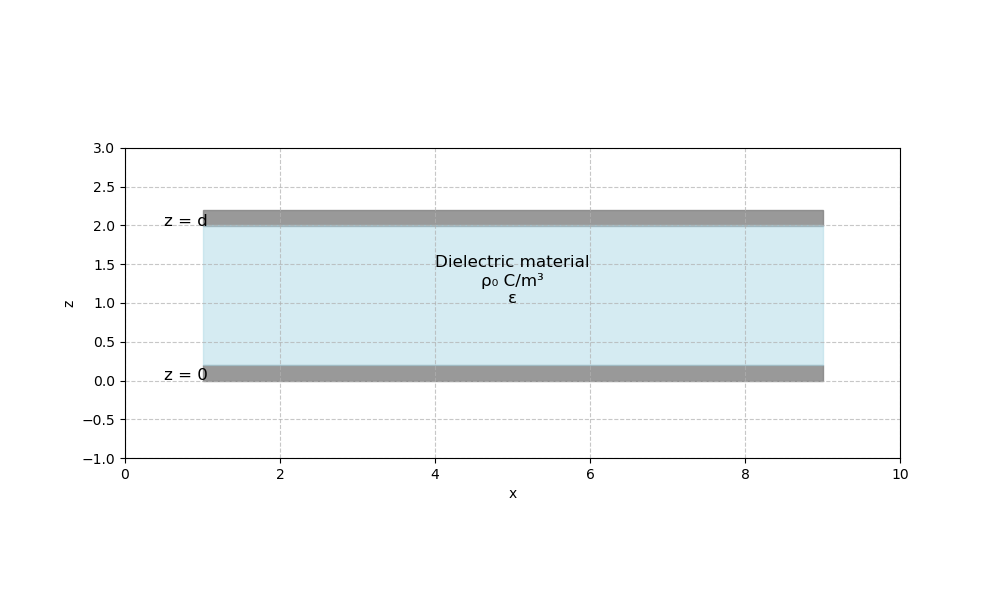
\includegraphics[width=0.7\textwidth]{./q8/fig.png}
    \end{center}
    \caption{Parallel Plate capacitor with dielectric}
\end{figure}


(a) By Poisson's equation (in a dielectric medium),
\begin{align*}
    \nabla^2 \phi = -\frac{\rho}{\epsilon_0}
\end{align*}

where $\phi$ is the potential field, $\rho$ is the charge density of the dielectric, $\epsilon_0$ is the permittivity of the free space.
\newline
We assume the plates of the capacitor to be infinite, and hence we assume a 1-D scenario \brak{\phi = \phi\brak{z}}.
\begin{align*}
    \nabla^2 \phi &= - \frac{\rho_0}{\epsilon_0}\\
    \implies \frac{\partial^2 \phi\brak{z}}{\partial z^2} &= - \frac{\rho_0}{\epsilon_0}\\
    \implies \frac{\partial \phi\brak{z}}{\partial z} &= - \frac{\rho_0}{\epsilon_0} z + c_1\\
    \implies \phi \brak{z} &= -\frac{\rho_0}{2\epsilon_0} z^2 + c_1 z + c_2
\end{align*}

where $c_1$ and $c_2$ are arbitrary constants.
\newline
Boundary conditions are given by $\phi\brak{0} = 0$, $\phi\brak{d} = 0$.
\begin{align*}
    \phi\brak{0} &= c_2 = 0\\
    \phi\brak{d} &= -\frac{\rho_0}{2\epsilon_0} d^2 + c_1 d + c_2 = 0\\
    \implies c_1 &= \frac{\rho_0 d}{2\epsilon_0}
\end{align*}
The potential field $\phi\brak{z}$ is now given by,
\begin{align*}
    \phi\brak{z} &= -\frac{\rho_0}{2\epsilon_0} z^2 + \frac{\rho_0 d}{2\epsilon_0}z\\
    \phi\brak{z} &= \frac{\rho_0}{2\epsilon_0} z\brak{d-z} \text{ , } 0 \leq z \leq d
\end{align*}

(b) Relation between $\mathbf{E}$ and $\phi$ is given by,
\begin{align*}
    \mathbf{E} = -\nabla \phi
\end{align*}
Gradient of $\phi$ is given by
\begin{align*}
    \nabla \phi &= \frac{\partial \phi}{\partial z} \hat{i} + \frac{\partial \phi}{\partial y} \hat{j} + \frac{\partial \phi}{\partial z} \hat{k}\\
    &= \frac{\partial \phi}{\partial z} \hat{i}\\
    &= \frac{\rho_0}{2\epsilon_0} \brak{\brak{d- z} - z}\\
    \implies \nabla \phi &= \frac{\rho_0}{2\epsilon_0}\brak{d - 2z} \hat{k}
\end{align*}
$\mathbf{E}$ is now given by,
\begin{align*}
    \mathbf{E} &= -\nabla \phi\\
    \implies \mathbf{E} &= \frac{\rho_0}{2\epsilon_0}\brak{2z - d} \hat{k} \text{ , } 0 \leq z \leq d
\end{align*}

(c) From part (a),
\begin{align*}
    \phi \brak{z} &= -\frac{\rho_0}{2\epsilon_0} z^2 + c_1 z + c_2
\end{align*}
In this case the, boundary conditions are given by $\phi\brak{0} = 0$, $\phi\brak{d} = V_0$.
\begin{align*}
    \phi\brak{0} &= c_2 = 0\\
    \phi\brak{d} &= -\frac{\rho_0}{2\epsilon_0} d^2 + c_1 d + c_2 = V_0\\
    \implies c_1 &= \frac{V_0}{d} + \frac{\rho_0 d}{2 \epsilon_0}
\end{align*}
Potential field $\phi\brak{z}$ is now given by,
\begin{align*}
    \phi \brak{z} &= -\frac{\rho_0}{2\epsilon_0} z^2 + \brak{\frac{V_0}{d} + \frac{\rho_0 d}{2 \epsilon_0}} z \text{ , } 0 \leq z \leq d
\end{align*}
Relation between $\mathbf{E}$ and $\phi$ is given by,
\begin{align*}
    \mathbf{E} = -\nabla \phi
\end{align*}
Gradient of $\phi$ is given by,
\begin{align*}
    \nabla \phi &= \frac{\partial \phi}{\partial z} \hat{i} + \frac{\partial \phi}{\partial y} \hat{j} + \frac{\partial \phi}{\partial z} \hat{k}\\
    &= \frac{\partial \phi}{\partial z} \hat{i}\\
    &= \brak{-\frac{\rho_0}{\epsilon_0} z + \brak{\frac{V_0}{d} + \frac{\rho_0d}{2\epsilon_0}}}\hat{k}
\end{align*}
$\mathbf{E}$ is now given by,
\begin{align*}
    \mathbf{E} &= -\nabla \phi\\
    \implies \mathbf{E} &= \brak{\frac{\rho_0}{\epsilon_0} z - \brak{\frac{V_0}{d} + \frac{\rho_0d}{2\epsilon_0}}} \hat {k}\text{ , } 0 \leq z \leq d
\end{align*}

\subsection*{Codes for simulations}

\subsubsection*{Q6 (a)}
\begin{minted}[
    frame=lines,
    framesep=2mm,
    baselinestretch=1.2,
    bgcolor=white,
    fontsize=\footnotesize,
    linenos
]{python}
import matplotlib.pyplot as plt
import numpy as np

epsilon_not = 8.85418e-12  # Permittivity of free space (F/m)
k = 1/(4*np.pi*epsilon_not)  # Coulomb constant

def E_Q(X, Y, q, pos):
    """
    Calculate the electric field at points (X,Y) due to a charge q at position pos.
    
    Parameters:
    X, Y: Grid of coordinates where the field is evaluated
    q: Charge value
    pos: (x,y) position of the charge
    
    Returns:
    Ex, Ey: Components of the electric field
    """
    Rx = X - pos[0] 
    Ry = Y - pos[1]
    norm = np.sqrt(Rx**2 + Ry**2)
    # Return the x and y components of the electric field using Coulomb's law
    return k*q*(X - pos[0])/norm**3, k*q*(Y - pos[1])/norm**3

def E(X, Y):
    """
    Calculate the total electric field at points (X,Y) due to four charges.
    
    The charges are arranged in a quadrupole configuration:
    - Positive charges at (0,1) and (0,-1)
    - Negative charges at (1,0) and (-1,0)
    
    Returns:
    Ex, Ey: Components of the total electric field
    """
    E1 = E_Q(X, Y, 1, (0, 1))
    E2 = E_Q(X, Y, 1, (0, -1))
    E3 = E_Q(X, Y, -1, (1, 0))
    E4 = E_Q(X, Y, -1, (-1, 0))
    
    # Return the sum of all field components
    return E1[0] + E2[0] + E3[0] + E4[0], E1[1] + E2[1] + E3[1] + E4[1]

x = np.linspace(-3, 3, 20)
y = np.linspace(-3, 3, 20)
X, Y = np.meshgrid(x, y)

U, V = E(X, Y)  # U = Ex, V = Ey
magnitude = np.sqrt(U**2 + V**2)

# Normalize the field components for the quiver plot
U_norm = U / magnitude
V_norm = V / magnitude

plt.figure(figsize=(6, 6))

# Create a quiver plot (vector field visualization)
# The color of the arrows represents the magnitude of the electric field
quiver_plot = plt.quiver(X, Y, U_norm, V_norm, magnitude, cmap='gnuplot')

# Add a colorbar to show the mapping between colors and field magnitudes
plt.colorbar(quiver_plot, label='Electric Field Magnitude')
plt.show()
\end{minted}

\subsubsection*{Q6 (b)}
\begin{minted}[
    frame=lines,
    framesep=2mm,
    baselinestretch=1.2,
    bgcolor=white,
    fontsize=\footnotesize,
    linenos
]{python}
import matplotlib.pyplot as plt
from matplotlib import cm
import numpy as np

# Create a new figure with a 3D subplot
fig = plt.figure(1)
ax = fig.add_subplot(111, projection='3d')

epsilon_not = 8.85418e-12  # Vacuum permittivity (F/m)
k = 1/(4*np.pi*epsilon_not)  # Coulomb constant

# Function to calculate electric potential due to a point charge
def V_Q(X, Y, q, pos):
    Rx = X - pos[0]
    Ry = Y - pos[1]
    norm = np.sqrt(Rx**2 + Ry**2)
    # Return potential using Coulomb's law
    return k*q/norm

# Function to calculate total electric potential from four charges
def V(X, Y):
    # Calculate potential from each of the four charges
    V1 = V_Q(X, Y, 1, (0, 1))    # Positive charge at (0,1)
    V2 = V_Q(X, Y, 1, (0, -1))   # Positive charge at (0,-1)
    V3 = V_Q(X, Y, -1, (1, 0))   # Negative charge at (1,0)
    V4 = V_Q(X, Y, -1, (-1, 0))  # Negative charge at (-1,0)

    return V1 + V2 + V3 + V4

# Create a grid of x and y coordinates
x = np.arange(-5, 6, 0.3)  # x values from -5 to 5 with step 0.3
y = np.arange(-5, 6, 0.3)  # y values from -5 to 5 with step 0.3
X, Y = np.meshgrid(x, y)   # Create 2D grid from x and y arrays

# Calculate the potential at each point in the grid
Z = V(X, Y)

# Create a surface plot with the 'gnuplot' colormap
surf = ax.plot_surface(X, Y, Z, cmap='gnuplot')

fig.colorbar(surf)
plt.show()
\end{minted}

\subsubsection*{Q5 (a)}
\begin{minted}[
    frame=lines,
    framesep=2mm,
    baselinestretch=1.2,
    bgcolor=white,
    fontsize=\footnotesize,
    linenos
]{python}
import matplotlib.pyplot as plt
import numpy as np

phi = np.arange(-20, 20, 0.1)
modF = np.sqrt((4 + 3*(np.cos(phi) + np.sin(phi)))**2 + 4)

plt.plot(phi, modF)
plt.xlabel('$\\phi$', fontsize=15)
plt.ylabel('$\\left|\\vec{F}\\right|$', fontsize=15)
plt.grid()
plt.show()
\end{minted}

\subsubsection*{Q5 (b)}
\begin{minted}[
    frame=lines,
    framesep=2mm,
    baselinestretch=1.2,
    bgcolor=white,
    fontsize=\footnotesize,
    linenos
]{python}
import matplotlib.pyplot as plt
import numpy as np

s = np.arange(-20, 20, 0.1)
modF = np.sqrt(4 + (40/(s**2 + 1) + 3*np.sqrt(2))**2)

plt.plot(s, modF)
plt.xlabel('$s$', fontsize=15)
plt.ylabel('$\\left|\\vec{F}\\right|$', fontsize=15)
plt.grid()
plt.show()
\end{minted}
\end{document}
